\documentclass[journal=jctcce,manuscript=article, layout=onecolumn]{achemso}
\usepackage[table]{xcolor}
\usepackage{amsmath}
\usepackage{graphicx}
\usepackage{float}
\graphicspath{ {./FIGs/} }

\author{Niccol\`{o} Ricardi}
\email{Niccolo.Ricardi@unige.ch}
\author{Cristina E. Gonz\'{a}lez-Espinoza}
\author{Tomasz Adam Weso\l{}owski}
\email{Tomasz.Wesolowski@unige.ch}
\affiliation[University of Geneva]
{Department of Physical Chemistry, University of Geneva, Geneva (Switzerland)}

\title[Negativity of the target density]
  {Negativity of the target density in practical Frozen-Density Embedding Theory based calculations}

\begin{document}

\begin{tocentry}

TOC to be made. Probably isosurfaces of target density.

\end{tocentry}


\begin{abstract}
Tentative abstract
\end{abstract}

%%%%%%%%%%%%%%%%%%%%%%%%%%%%%%%%%%%%%%%%%%%%%%%%%%%%%%%%%%%%%%%%%%%%%
%% Start the main part of the manuscript here.
%%%%%%%%%%%%%%%%%%%%%%%%%%%%%%%%%%%%%%%%%%%%%%%%%%%%%%%%%%%%%%%%%%%%%
\section{Introduction}
\begin{itemize}
 \item ${E}_{v_A,v_B}^{FDET}[\Psi_{A},\rho_B] = \langle\Psi_{A}\vert \hat{H}_A\vert \Psi_{A}\rangle +E^{HK}_{v_B}[\rho_B]+E_{v_{A},v_{B}}^{int} + \Delta F[\rho_A] + \int
{\rho_A(\vec{r})v_B(\vec{r})}d\mathbf{r} + \int\int \frac{\rho_A(\vec{r})\rho_B(\mathbf{r}')} {\left\vert \mathbf{r}-\mathbf{r}'\right\vert}d\mathbf{r}'d\mathbf{r}  
+ {E}_{xcT}^{nad}[\rho_A,\rho_B] +\int
{\rho_B(\vec{r})v_A(\vec{r})}d\mathbf{r}$
 \item ${E}_{v_A,v_B}^{FDET}[\Psi_{A}^{o},\rho_B]=E_{v_{AB}}^{HK}[\rho_A^{o}+\rho_B] \ge E_o$
%  \item shape of embedding potential
 \item if $\rho^t(\mathbf{r}) = \rho_o(\mathbf{r}) - \rho_B(\mathbf{r})$ is not positive for $\forall \mathbf{r}$, then it is not v-representable, and there is no possible embedding potential that can lead to $\rho^t(\mathbf{r})$
 \item the aim of this manuscript is to assess if there is a relation between some measurement of the negativity of $\rho^t(\mathbf{r})$ and ${E}_{v_A,v_B}^{FDET}[\Psi_{A},\rho_B]$
%  \item if $\delta \rho_B (\mathbf{r})$ so that the extent of violation is reduced, the induced change in energy has to be non-positive ($\delta E^{FDET}[\Psi_A,\rho_B; v_B] \leq 0$) 
%  \item if we somehow measure the extent of non-negativity, and this is reduced, the energy should also lower. This is true unless:
%  \begin{itemize}
%   \item the violation reduces in a region of the space and increases somewhere else, with a larger energy effect in the latter than the former.
%   \item the contributions of the other sources of error (approximate functionals and potentials, basis set expansion) do not change significantly
%  \end{itemize}
 \item polarization and charge transfer can be expected to influence the extent of violation of the target density. This manuscript also aims at assessing the relation between negativity of the target density and phenomena such as polarization and charge transfer
 \item Why these 4 systems
\end{itemize}

\subsection{Measurement of the violation}
\begin{itemize}
  \item $ M[\rho_{t}] = -\int \rho^{t}(\vec{r})\cdot \Theta(-\rho^{t}(\vec{r})) \ d\vec{r}$
 \end{itemize}

\section{Approximate FDET-based methods}
\begin{itemize}
 \item HF embedding
 \item Taylor approach for MP
\end{itemize}

 \section{Computational Details}
\subsection{subsection title to decide}
\begin{itemize}
%  \item We study each of the 4 systems individually so that the changes in other error contributions are minimized
%  \item The energy effect of density is far from easy
 \item choices of $\rho_B(\mathbf{r})$ labels for different densities
 \item ME and SE
 \item in-house iterative procedure (Nico's fork of Alex's CCJob)
 \item Qchem version
 \item basis set, functionals
 \item $ P[\rho_{AB}^{ref}, \rho_{AB}^{FDET}] = \frac{1}{2} \cdot \int \lvert \rho_{AB}^{ref}(\vec{r}) - \rho_{AB}^{FDET}(\vec{r}) \rvert \ d\vec{r}$
 \item pyscf to perform integration of M and P
\end{itemize}

\section{Results and discussion}
\subsection{Monomer Expansion}
\begin{figure}[H]
\centering
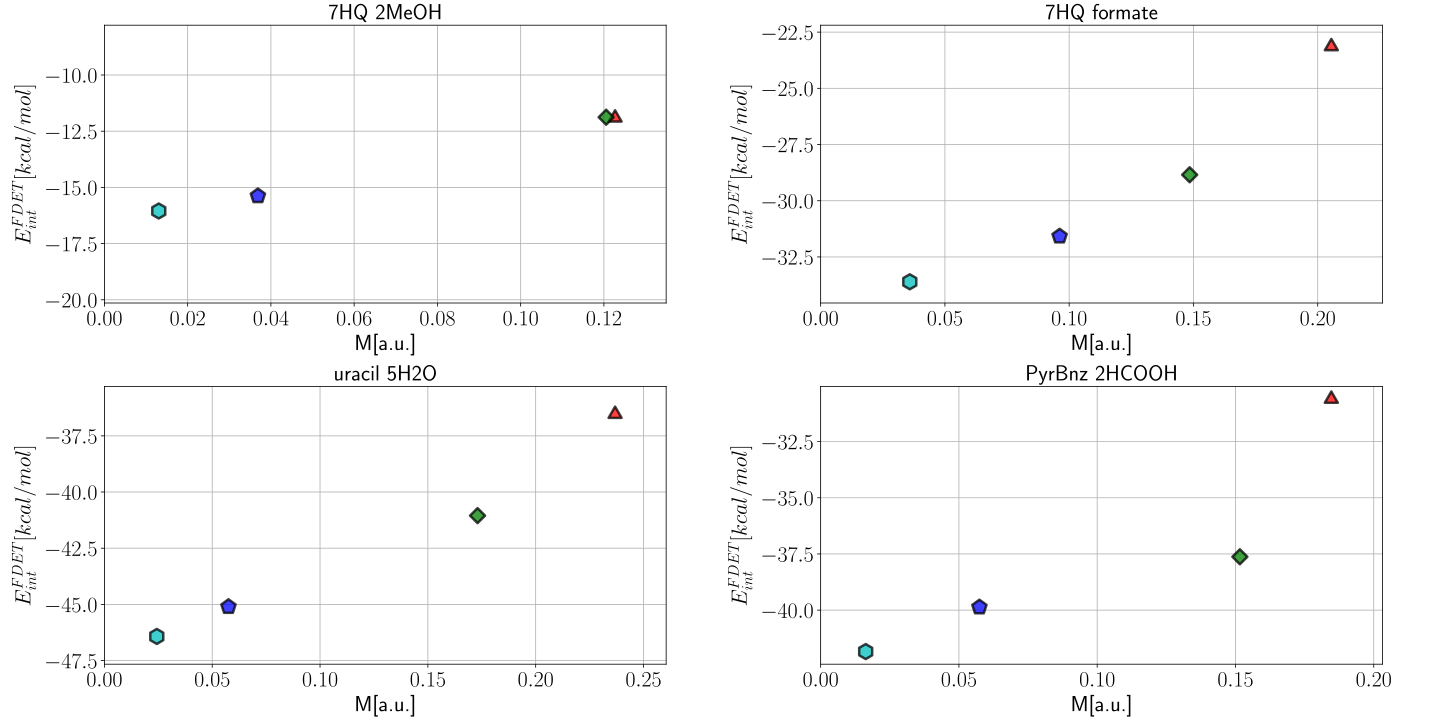
\includegraphics[width=1.0\linewidth]{M_vs_HF.png}
\caption{Integrated negative density $M$ versus $E_{HF}$, for monomer expansion calculations}
\label{fig:M_VS_HF}
\end{figure}
M vs $E_{HF}$
\begin{itemize}
 \item When M decreases, so does the HF energy
 \item When we somehow prepolarize, we obtain a decrease in M, and the behavior is sensible (Mulliken $<$ ChelPG $<$ Freeze and Thaw, Mulliken sometimes no improvement)
\end{itemize}
M vs P
\begin{figure}[H]
\centering
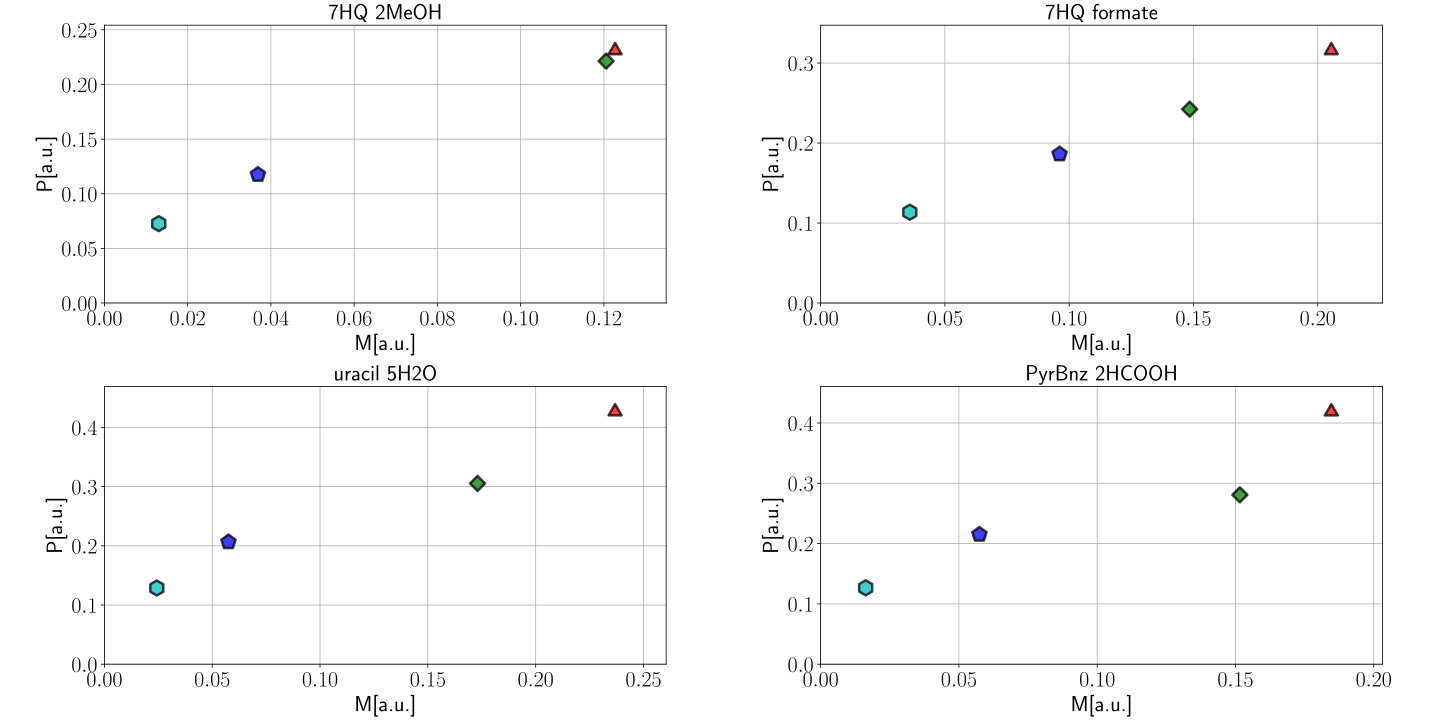
\includegraphics[width=1.0\linewidth]{M_vs_P.png}
\caption{Integrated negative density $M$ versus total density error $P$, for monomer expansion calculations}
\label{fig:M_vs_P}
\end{figure}
\begin{itemize}
 \item When M decreases, so does the density error $P$
\end{itemize}
M vs $E_{MP}$
\begin{figure}[H]
\centering
\includegraphics[width=1.0\linewidth]{M_vs_MP.png}
\caption{Integrated negative density $M$ versus $E_{MP}$, for monomer expansion calculations}
\label{fig:M_vs_MP}
\end{figure}
\begin{itemize}
 \item When M decreases, so does the MP energy (obtained according to Wesolowski 2020)
 \item Small deviation from expected behavior is small and can be explained by the approximate correlation treatment, the approximate external potential, and the incomplete basis set
 \item Freeze and Thaw SE improvement for 7HQ formate and XVI 2HCOOH
\end{itemize}



\subsection{Freeze and Thaw cycles}
N vs $E_{HF}$, SE
\begin{figure}[H]
\centering
\includegraphics[width=1.0\linewidth]{SE_cycles_N_vs_HF.png}
\caption{$E^{FDET}[\Psi_A,\rho_B; v_B]$ with fully self-consistent calculations(blue ``X''), linearized FDET (red ``+''), and not self consistent direct calculation (red dots).}
\label{fig:N_vs_HF_SE}
\end{figure}
\begin{itemize}
 \item the first freeze and thaw iteration leads to the largest energy decrease
 \item after 1-2 freeze and thaw iterations the energy is almost equal to the fully converged one
 \item the linearization is extremely accurate, $\Delta^{lin}$ decreases during freeze and thaw, and finally reaches zero
 \item same findings for ME (cf. SI), why we showed SE
\end{itemize}

\section{Conclusions}
\begin{itemize}
 \item the negativity of the target density clearly increases $E^{FDET}[\Psi_A,\rho_B; v_B]$
 \item prepolarization techniques reduce negativity, and consequently $E^{FDET}[\Psi_A,\rho_B; v_B]$
 \item the negativity of the target density is a sizeable error contribution. Error analysis should account for this.
 \item Single-state properties require some type of prepolarization
 \item ESP-derived charges are a well-performing tradeoff between computation time and accuracy
\section{Perspective and outlook}
 \item the error on excitation properties depends on the difference of negativity violation $\Delta M$. This implies:
    \begin{itemize}
     \item no-prepolarization can be expected to be much better than for single-state properties
     \item the effect of prepolarization is hard to predict, and knowledge of the system is necessary
    \end{itemize}

\end{itemize}

\begin{acknowledgement}
The authors thank funding xyz.
\end{acknowledgement}

\begin{suppinfo}
The data is provided in csv.
\begin{itemize}
  \item Filename: data as comma separated values. The labels are explaind below:
  \begin{itemize}
   \item label: explanation
  \end{itemize}


\end{itemize}

\end{suppinfo}

%%%%%%%%%%%%%%%%%%%%%%%%%%%%%%%%%%%%%%%%%%%%%%%%%%%%%%%%%%%%%%%%%%%%%
%% The appropriate \bibliography command should be placed here.
%% Notice that the class file automatically sets \bibliographystyle
%% and also names the section correctly.
%%%%%%%%%%%%%%%%%%%%%%%%%%%%%%%%%%%%%%%%%%%%%%%%%%%%%%%%%%%%%%%%%%%%%
\bibliography{achemso-demo}

\end{document}
